People Gazetteer as defined in Section~\ref{sec:introduction} consists of tuples of person names along with list of documents in which they occur and their corresponding topics. It is developed as an organized structure that can facilitate the process of detection of influential persons from the dataset in an efficient and easy way. This section describes the 2-step process of construction of the People Gazetteer by
a) Extraction of person names from the news articles dataset using Named Entity Recognition in  Section~\ref{ner} and
b) Assignment of topics to news articles using LDA topic detection in  Section~\ref{topic detection}.
Output of People gazetteer developed using these steps is presented in Section ~\ref{gaz:result}.

\subsection{Person Named Entity Recognition (PNER)}
\label{ner}


\subsubsection{Definition}
NER (Named Entity Recognition) refers to classification of elements in text into pre-defined categories such as the names of persons, organizations, locations, expressions of times, quantities, monetary values, percentages, etc. It can also be considered as a sequence labeling problem that predicts label of each element of the text  based on the adjacent element labels.

Person Named Entity Recognition (PNER) can be defined as the process of NER that marks up only person names that occur in the text. It is done in two phases: chunking ,i.e., segmentation of text for name detection followed by classification of the name by the type of entity it belongs to (person,organization,location,etc.).

PNER is required in this research so as to extract all person name entities occurring in the complete dataset and then identify influential person entities among them through development of the People Gazetteer. 
PNER aids in the development of People Gazetteer by first extracting a list of all person names occurring in the dataset followed by creation of a Person-Article list where each person is linked with the articles in which he/she occurs.

\subsubsection{Methodology}
\label{ner:method}

While earlier NER models were rule-based or dictionary-based that use linguistic grammar based techniques, current studies use statistical sequential models that predict labels for sequential data using probabilistic techniques. They also require labeled training data with all of the entities of interest and their types. Statistical machine learning models like Hidden Markov Models or MaxEnt Markov Models follow a generative or discriminitave approach respectively. In the generative approach, a joint probability distribution over input and output variables is modeled assuming independent features and considering future observations into account while the discriminative approach models conditional distribution directly, without assuming independent features or considering future observations.
 The linear chain CRF (Conditional Random Field)  sequence model for NER is a combination of generative and discriminative approach and is considered state of the art for performing  NER (\cite{mccallum2003early, finkel2005incorporating, sutton2011introduction}). The model can be viewed as a conditionally trained finite state machine which is used to find the possible label sequence given an input sequence and learning. It combines features of discriminative and generative models by relaxing the assumption that features are independent and considers future observations into account during sequential labeling.

The Stanford CRF-NER\footnote{http://nlp.stanford.edu/software/CRF-NER.shtml} is used for PNER in this research. It can perform NER for 3 classes: Person, Organization and Location and is based on linear chain CRF sequence models.
 It is trained across several newspaper corpora and is fairly robust across multiple domains and performs best when compared to some other open source NER systems which is the reason it has been used for this study. As illustrated by Rodriquez et. al \cite{rodriquez2012comparison}, Stanford NER gave overall the best performance across 2 OCR datasets, and was most effective for PNER when compared with 3 other open source NER systems.

%NO NEED OF THIS FIGURE
%\subsubsection{PNER Results}
%\label{ner:results}
%\begin{figure*}
 % \centering
%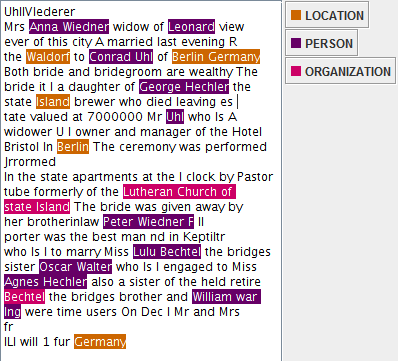
\includegraphics{NER1}
%\caption{NER on a sample news article}
%\label{figure:sample}
%\end{figure*} 




%NER on a sample news article from the dataset can be seen in Figure~\ref{figure:sample}.
 Stanford NER recognizes a person's full name as separate names by default which is rectified by combining these multi-term entities into single person entities. For example, the person name ``John Smith" is recognized as two separate person entities which we combine to form a single multi-term person entity.
Person names tagged with ``PERSON" category are stored while running NER on the dataset.
Whenever a multi-term person name (number of terms in the person name must be greater than 1) occurs in a document, the person entity's name along with the document name is stored to obtain tuples of person names with their document occurrences in a Person-Article List.
The Stanford NER takes 25 minutes to run on the complete news dataset of 14020 articles extracting a total of 36362 person entities.  

%\begin{table*}
 % \begin{center}
%\begin{tabular}{|l|l|l|}
   % \hline
%\textbf{No. of Person Entities} & \textbf{No. of articles} \\ \hline
%36615                  & 1               \\ \hline
%1122                   & 2               \\	\hline
%329                    & 3               \\	\hline
%123                    & 4               \\	\hline
%87                     & 5               \\	\hline
%48                     & 6               \\	\hline
%29                     & 7               \\	\hline
%19                     & 8               \\	\hline
%16                     & 9               \\	\hline
%5                      & 10              \\	\hline
%4                      & 11              \\	\hline
%6                      & 12              \\	\hline
%4                      & 14              \\	\hline
%3                      & 15              \\	\hline
%2                      & 16              \\	\hline
%1                      & 17              \\	\hline
%1                      & 18              \\	\hline
%3                      & 19              \\	\hline
%1                      & 20              \\	\hline
%1                      & 21              \\	\hline
%1                      & 22              \\	\hline
%1                      & 23              \\	\hline
%1                      & 27              \\	\hline
%1                      & 29              \\	\hline
%1                      & 31              \\	\hline
%1                      & 34              \\	\hline
%1                      & 35              \\ 	\hline
%\end{tabular}
%\end{center}
%\caption{Table showing output of PNER on 14020 articles}
%\label{table:Table1}
%\end{table*}


We divide the people entities extracted into following categories so that separate analysis can be done for each category:
\begin{itemize}
 \item \textbf{Marginally Influential}: This category includes all person entities with occurrence in less than 4 news articles. (36004 person entities )
\item \textbf{Medium Influential}: This category includes all person entities with occurrence from 4 to 15 news articles. (344 person entities) 
\item \textbf{Highly Influential} : This category includes all person entities with occurrence in 16 or more news articles. (14 person entities)
\end{itemize}
Figure ~\ref{figure:res} shows the statistics for each of these categories of persons extracted from the dataset. These categories have been chosen manually simply based on the number of articles of occurrence of a person entity and do not directly lead to the conclusion of a person entity with large number of articles being influential.

\begin{figure*}
  \centering
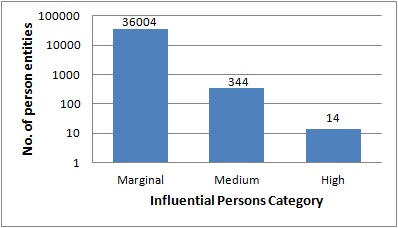
\includegraphics{IPChart}
\caption{Log Scale plot showing number of persons extracted for each influential person category after PNER from the dataset}
\label{figure:res}
\end{figure*} 


\subsection{Topic Detection}
\label{topic detection}

 Topic models are algorithms for discovering the main topics that occur across a large and otherwise 
unstructured collection of documents and can organize the collection according to the discovered topics.
Here, a topic refers to a set of words which describe what any document is about.
 A topic model examines the set of documents and discovers based on the statistics of the words in each, what the topics might be and what each document's balance of topics is.
Documents are considered as a mixture of topics and each topic a probability distribution over words.
 Topic detection is the process of identifying topics in a document collection using a topic model. 
%A simple example of topic model illustrated by \cite{blei2012probabilistic} can be seen in Figure~\ref{figure:example}.

Topic detection is essential to this research in order to determine the topics of individual news articles that a person entity occurs in so that the person entity can be linked to the documents in which he/she occurs along with their respective topics.

%\begin{figure*}
%\begin{center}
%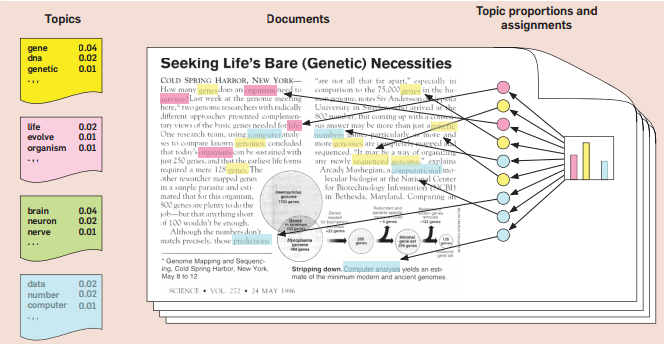
\includegraphics[scale=0.8]{topicmodel}
%\caption{Simple topic modelling approach for a single article\cite{blei2012probabilistic}}.
%\label{figure:example}
%\end{center}
%\end{figure*} 


\subsubsection{Topic Detection Model}
\label{topic detection:model}
\paragraph\textbf{Latent Dirichlet Allocation (LDA) Model}

LDA is a generative probabilistic model in which each document is modeled as a finite mixture over an underlying set of topics and each topic, in turn, is modeled as an infinite mixture over an underlying set of topic probabilities\cite{blei2003latent}. In other words, documents exhibit multiple topics and each topic is a distribution over a fixed vocabulary.
The LDA model can be briefly reviewed as follows:


Given an input corpus of $D$ documents with $K$ topics, each topic being a multinomial distribution over a vocabulary of  $W$ words, the documents are modeled by fitting parameters `${\Phi}$' and `${\Theta}$'. `${\Phi}$' is a matrix of size $D \times K$ in which each row is a multinomial distribution of document $d$  indicating the relative importance of words in topics. ${\Theta}$ is the matrix of size $W \times K$ with each column a multinomial distribution of topic $j$ and corresponds to the relative importance of topics in documents.

Given the observed words x = ${x_i}_j$, LDA inference is done by computing the
posterior distribution over the latent topic assignments z = ${z_i}_j$, the mixing proportions ${\Theta_j}$  and the
topics ${\Phi_k}$.  The inferencing is either done using variational bayesian methods or Gibbs sampling which involves integration and sampling of latent variables.
However, the simple LDA approach can take several days to run over a large corpora.


\paragraph\textbf{Distributed LDA Model}
 
The simple LDA method takes a long time for topic modeling which is why the distributed version suits large datasets such as ours. The data is partitioned across separate processors and inference is done in a parallel, distributed fashion. 

The Approximate Distributed LDA (AD--LDA) model as proposed by \cite{newman2009distributed} uses distributed computation where total dataset $D$ is distributed equally among multiple $P$ processors. Initialization involves data and parameters distribution to each processor and random assignment of topics so that each processor has its own copy of words $x_p$, topics $z_p$, word topic counts ${{{N_w}_k}_p}$ and topic counts ${{{N_k}_j}_p}$. 
The topic model inferencing then uses simultaneous local Gibbs sampling approach on each processor for a pre-decided number of iterations to reassign topic probabilities $z_p$, word topic ${{N_w}_k}_p$ and topic counts ${{N_k}_j}_p$.
Global update is performed after each pass by using a reduce-scatter operation on word topic count ${{N_w}_k}_p$ to get a single set of counts and obtain final topic assignments.
The model requires user set parameters before inferencing such as number of processors/threads for parallel sampling of data, number of iterations of Gibbs sampling, number of topics and Dirichlet parameters. 

\subsubsection{Topic Models Evaluation}

 Different topic models can be evaluated using the metric of ``Perplexity" which can be defined as how surprised a trained model is when given a held out test data. It has been used in \cite{newman2009distributed} and \cite{blei2003latent} for evaluating the topic detection models under different parameter settings. Perplexity can be calculated using the following formula:

$$Perplexity= \exp(-\dfrac{\text{Log Likelihood of held-out test set}}{\text{Number of tokens in held-out test set}})$$


Here, held-out test set refers to the fact that complete dataset is split into two parts: one for training and the other for testing. The test set is taken as the held-out set for which perplexity is calculated. The document mixture is learned using the training data and log probability of the test data containing unseen documents is computed using the model developed.

Perplexity is a decreasing function of the log likelihood of the unseen documents as can be seen from its formula and lower the perplexity, better is the topic model.

\subsubsection{Results}
\label{topic detection:result}

The AD-LDA model as described in \cite{newman2009distributed} and implemented in the Mallet\cite{McCallumMALLET} toolkit (known as PLDA model) is used for topic detection over the complete dataset of 14020 news articles. 
Several topic models are first evaluated with different parameter settings in order to pre-decide the number of iterations, processors and topics for the final topic model to be used.


%After training, parameter settings as number of topics varying from 10 to 100, number of iterations from 100 to 500 and number of processors from 1 to 8, the log likelihood of held-out test dataset is calculated along with number of tokens in it to obtain perplexity.

\begin{figure*}
\begin{center}
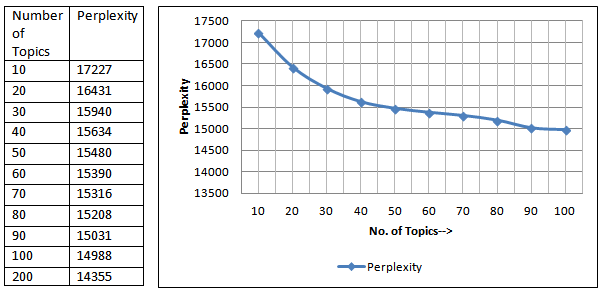
\includegraphics{topicperplex2}
\caption{Test Set Perplexity versus Number of Topics for a random $90-10$ split of the data. The maximum number of words in each topic is $20$, number of iterations $500$ and the number of processors $4$ for this experiment.}
\label{figure:perplex}
\end{center}
\end{figure*}

Perplexity is calculated by splitting the data into 90\% for training and rest 10\% for testing. 
Figure~\ref{figure:perplex} shows the variation of the test perplexity versus the number of topics for one random $90-10$ split of the data\footnote{We also vary the number of iterations from 100 to 500 and number of processors from 1 to 8 to study their effect on perplexity. However the number of topics is most influenced by perplexity and hence the other results are not presented here.}. The maximum number of words in each topic is set to $20$, number of iterations $500$ and the number of processors $4$ for this experiment. It exhibits a decreasing perplexity with increase in number of topics. Typically, the number of topics should be chosen as high as possible in order to consider a better model with low perplexity but the model with high number of topics also takes longer to run on a large dataset. The number of topics is set to a value from where further increase in number of topics does not lead to a large decrease in perplexity. We choose the number of topics as $30$ and $100$ and demonstrate their effect on the influential people detection.

From the various topic models and parameter settings, the variability in perplexity with respect to the number of topics has been found to be much greater than the variability due to the number of processors or number of iterations. This is why two values of number of topics are experimented further while number of processors and number of iterations are kept fixed. The number of iterations of Gibbs sampling still need to be above the typical burn-in period of $200$ which is why $500$ is chosen as the parameter value for number of iterations. Number of threads/processors is similarly taken as 4 as least training time is obtained with this parameter value. 

The two models from topic detection are thus used with following parameters:
\begin{enumerate}
 \item \textbf{30 Topics LDA Model} : Number of topics = 30, Number of iterations = 500, Number of threads=4
 \item \textbf{100 Topics LDA Model} : Number of topics = 100, Number of iterations = 500, Number of threads=4
\end{enumerate}
The first model takes 7.5 minutes for training while the second one takes 8.6 minutes.
%The set of 30 topics obtained through the first model are illustrated in Table~\ref{table:topicwords} and the other model with 100 topics in Appendix Table~\ref{long}. 
Some of the topics words from the topic models can be easily identified to belong to the following topics: music performance, court events, elections and government and shipping.

Topic modeling gives as output, for each article in the dataset, a set of topics with their probability distribution score for the article. The topic with highest topic probability score is associated with each article in the dataset to obtain an Article-Topic List.


\subsection{People Gazetteer Output }
\label{gaz:result}

\begin{figure*}
\begin{center}
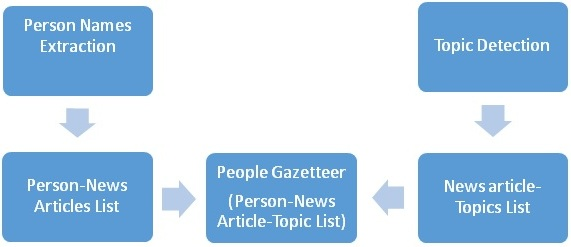
\includegraphics{gaz}
\caption{Procedure for development of People Gazetteer}
\label{figure:gaze}
\end{center}
\end{figure*}

The procedure of development of people gazetteer can be seen in Figure~\ref{figure:gaze}.The list of articles obtained for each person entity after application of PNER (Person-Article List) and highest scoring topic assigned to each article during Topic Detection (Article-Topic List) are combined to obtain People Gazetteer. In each tuple of the gazetteer, a person entity gets associated with its list of articles in which it occurs and where each article is further associated with its corresponding highest scoring topic. 

Two people gazetteers are finally developed, each corresponding to the two model settings of 30 Topics LDA Model and 100 Topics LDA Model, respectively. Both gazetteer consist of a list of named entities along with the articles of their occurrence and topic associated with each article. A snapshot of the people gazetteer using 30 Topics LDA Model can be seen in Figure~\ref{figure:gazette} where each person entity is followed by a document list consisting of a Document ID and its corresponding Topic ID. A similar people gazetteer is also obtained using 100 Topics LDA Model. Both People Gazetteers are further used in Section~\ref{influential} for detecting and ranking influential person entities from them.
\begin{figure*}
\centering
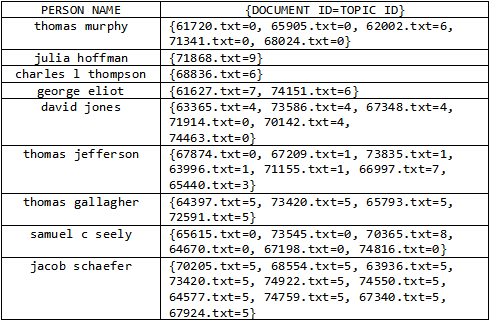
\includegraphics{gazetteer}
\caption{Snapshot of People Gazetteer with Person names, Document list of occurrence and their corresponding Topic ID}
\label{figure:gazette}
\end{figure*} 
